\section{Text translation using pre-trained
Transformers}\label{text-translation-using-pre-trained-transformers}

\begin{lstlisting}[language=Python]
from transformers import MarianMTModel, MarianTokenizer

model_name = "Helsinki-NLP/opus-mt-en-es"
tokenizer = MarianTokenizer.from_pretrained(model_name)
model = MarianMTModel.from_pretrained(model_name)
\end{lstlisting}

\begin{lstlisting}
/opt/venv/lib/python3.10/site-packages/tqdm/auto.py:21: TqdmWarning: IProgress not found. Please update jupyter and ipywidgets. See https://ipywidgets.readthedocs.io/en/stable/user_install.html
  from .autonotebook import tqdm as notebook_tqdm
/opt/venv/lib/python3.10/site-packages/transformers/models/marian/tokenization_marian.py:194: UserWarning: Recommended: pip install sacremoses.
  warnings.warn("Recommended: pip install sacremoses.")
\end{lstlisting}

First, we import the \lstinline{MarianMTModel} and
\lstinline{MarianTokenizer} classes from the
\lstinline{transformers} module, which is a popular Python
library for working with transformer-based models such as BERT, GPT, and
MarianMT.

Next, we set the \lstinline{model_name} variable to
\lstinline{Helsinki-NLP/opus-mt-en-es}, which is the name
of the pre-trained model that will be used for English-to-Spanish
translation. Read more about this pre-trained model
\href{https://huggingface.co/Helsinki-NLP/opus-mt-en-es}{here}.

The \lstinline{MarianTokenizer} class is then used to
instantiate a \lstinline{tokenizer} object, which will be
used to tokenize the input text before passing it to the model.

Similarly, the \lstinline{MarianMTModel} class is used to
instantiate a translation \lstinline{model} object. The
model object is initialized with the pre-trained weights of the
English-to-Spanish translation model specified by
\lstinline{model_name}.

\begin{lstlisting}[language=Python]
import warnings
warnings.filterwarnings('ignore')

def translate(model, tokenizer, text: str) -> str:
    """
    :param text: English text
    :return: Spanish text (translated from the English input)
    """
    # Tokenize the input text
    inputs = tokenizer(text, return_tensors="pt")
    # Generate the corresponding Spanish translation
    outputs = model.generate(**inputs)
    # Decode the translated text
    translated = tokenizer.decode(outputs[0], skip_special_tokens=True)
    return translated

text = "Hello, how are you doing today?"
translated = translate(model, tokenizer, text)
print(translated)
\end{lstlisting}

TODO:

Try building a text translation application that can detect and
translate text from different languages. You can use the pre-trained
models available
\href{https://huggingface.co/models?pipeline_tag=translation&sort=downloads}{here}.

\section{GPT3 and ChatGPT}

\subsection{GPT-3}

\begin{itemize}
    \item GPT-3 is a language model developed by OpenAI based on transformer architecture.
    \item It was released in June 2020 and is known for its impressive performance on various language tasks.
    \item GPT-3 is trained on over 45 terabytes of text data and has 175 billion parameters.
    \item The model is pre-trained on a language modeling objective, which allows it to learn a general understanding of language, including syntax, semantics, and context.
    \item GPT-3's architecture is based on the transformer, which consists of a stack of transformer layers with multiple attention heads.
    \item The model incorporates several innovations, including relative positional encoding and a mixture of experts to specialize in different areas of language processing.
\end{itemize}
You can use GPT-3 using API developed by OpenAI by creating an account on the \href{https://platform.openai.com/overview}{\textbf{OpenAI website}}. \newline

We also recommend exploring \href{https://platform.openai.com/playground}{\textbf{Open AI playground(opens in a new tab)}} to test GPT-3 and other models for various NLP tasks.

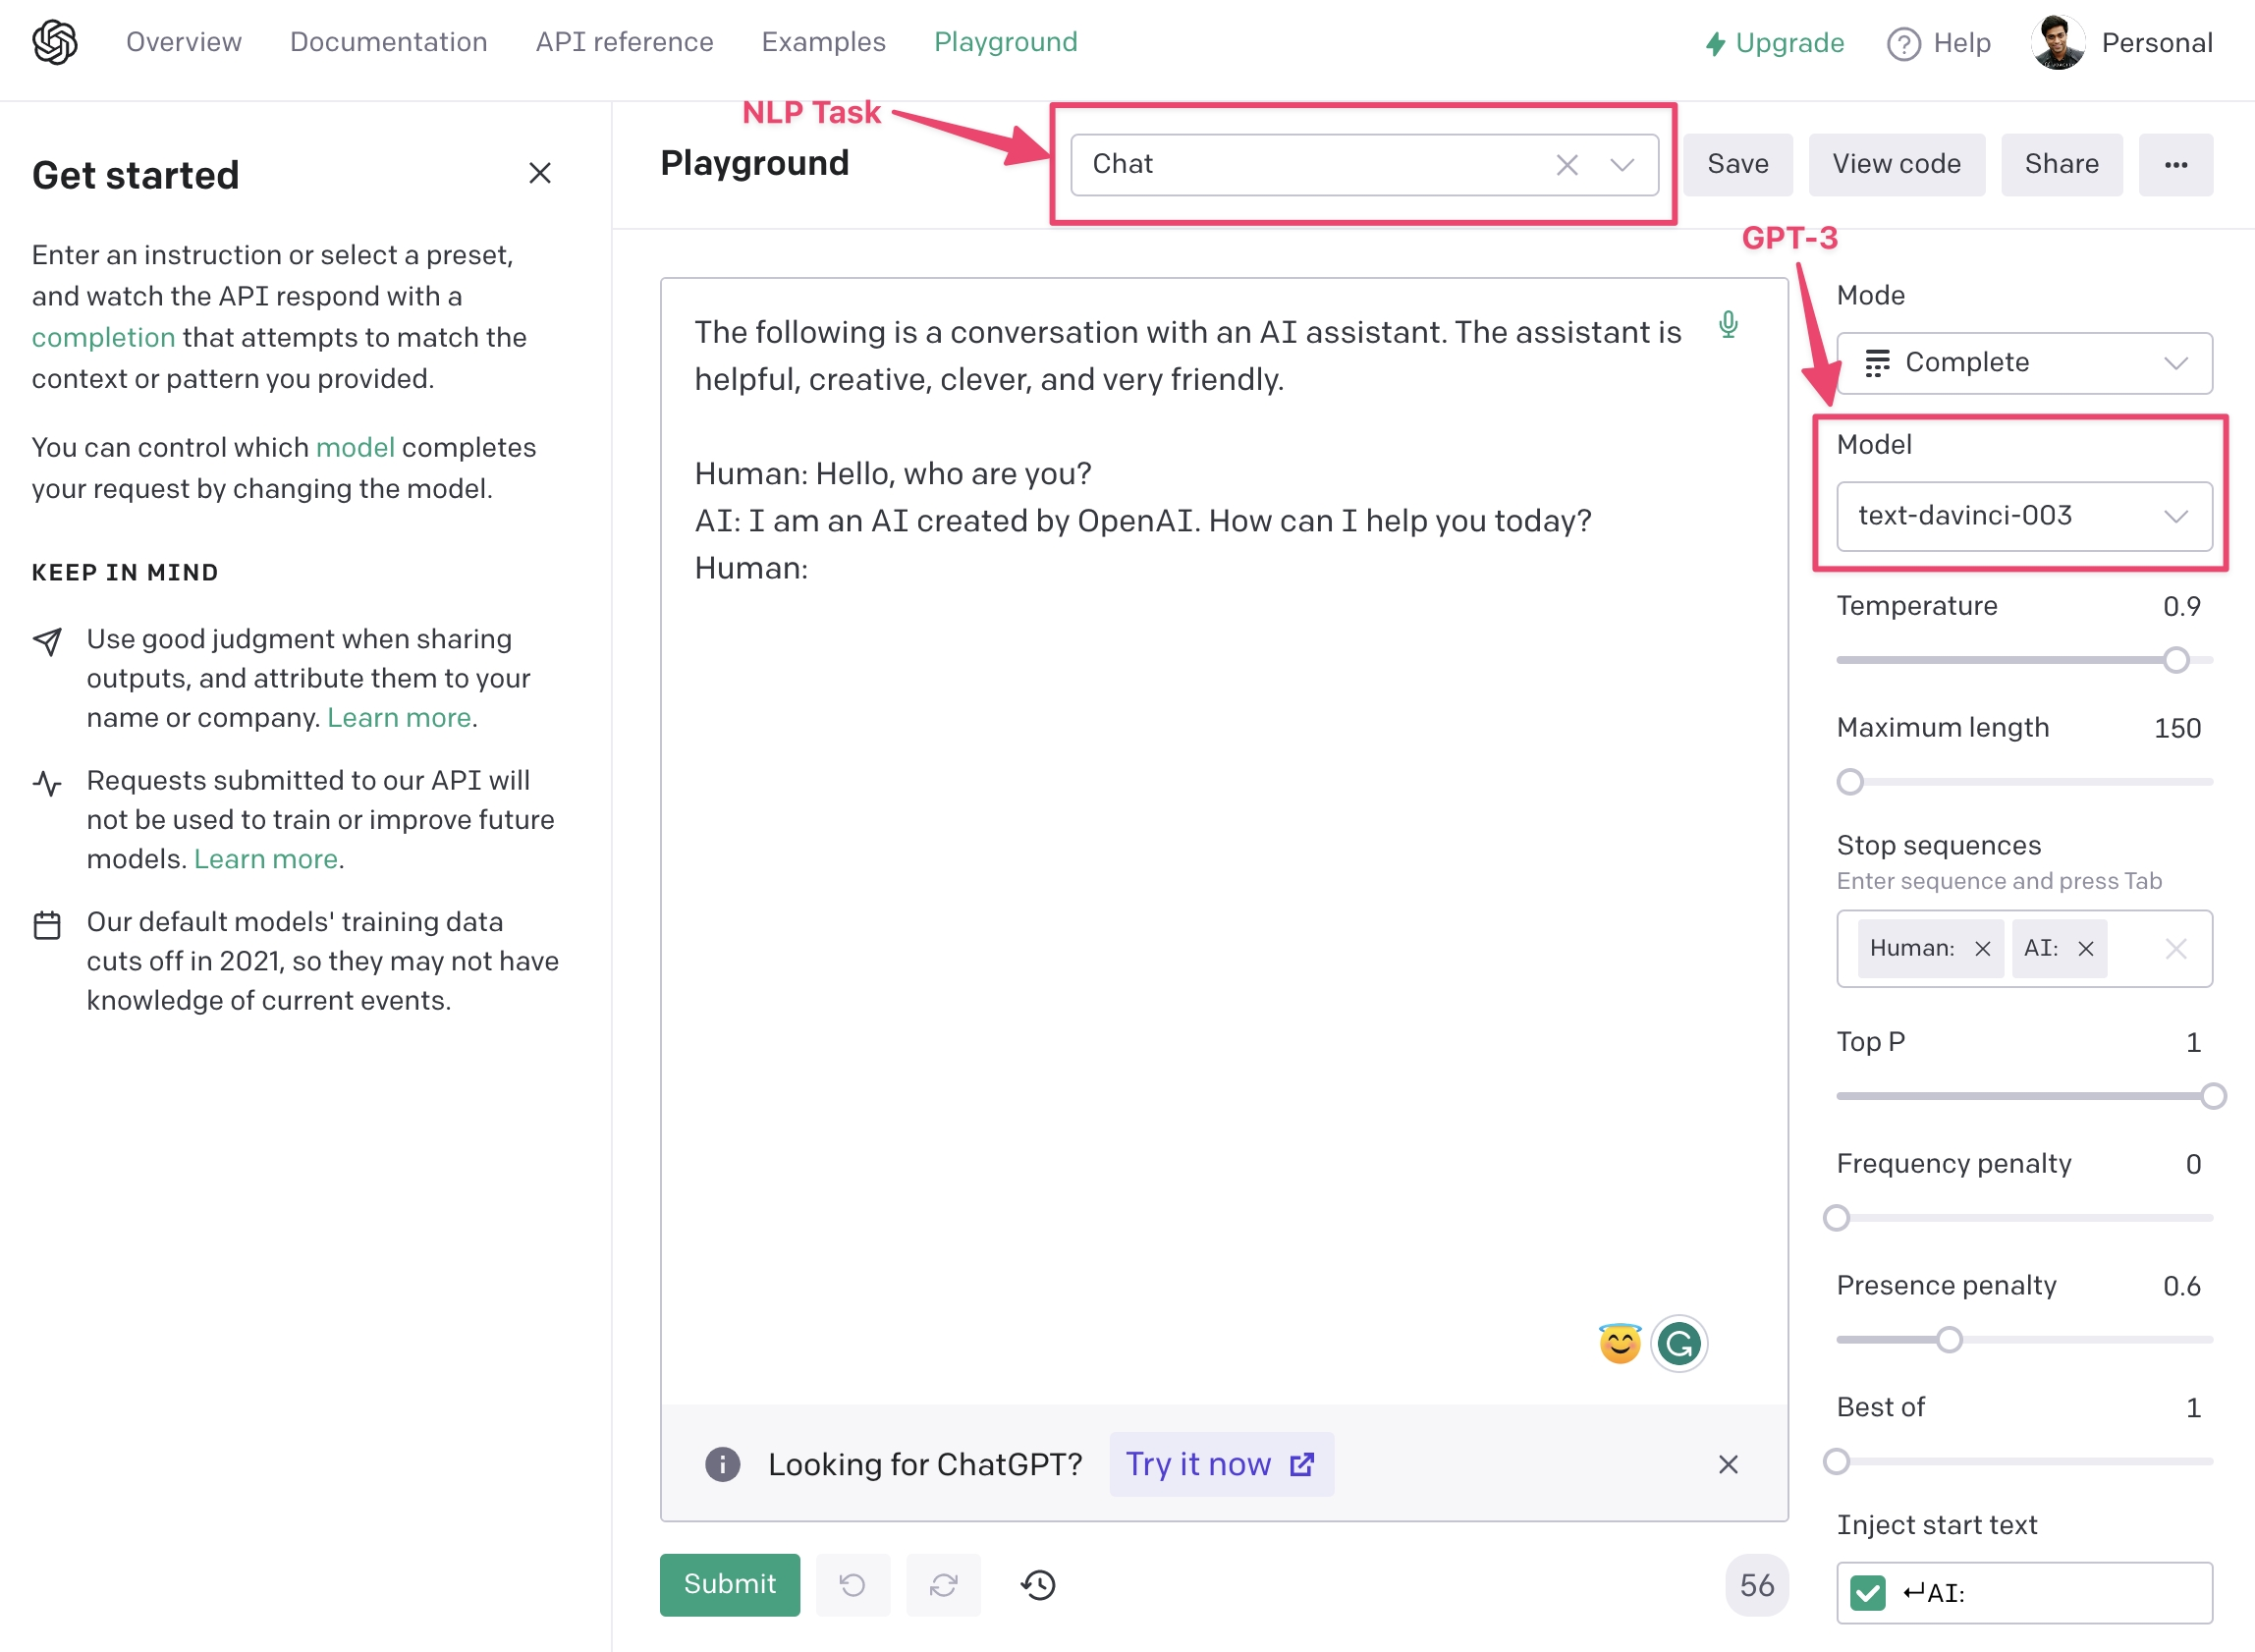
\includegraphics[width=1\linewidth]{img//rnn//transformers/open_ai_playground.jpeg}
\captionof{figure}{Open AI Playground}

Click on \textbf{View Code} if you would like to integrate this model in your application.

\subsection{ChatGPT}

\begin{itemize}
    \item ChatGPT is a large language model developed by OpenAI based on the GPT-4 architecture.
    \item It is an NLP tool that can generate human-like responses to textual input.
    \item ChatGPT has been trained on a vast corpus of text data and can understand the nuances of language, including grammar, syntax, and context.
    \item It can be used for chatbots, customer service, virtual assistants, language learning, tutoring, and more.
    \item ChatGPT has a vast knowledge base and can provide answers to a wide range of questions, making it a valuable resource for researchers, students, and professionals.
    \item Its ability to understand the context of the conversation and generate relevant responses has made it popular for companies looking to automate their customer service and support functions.
    \item ChatGPT's conversational abilities are continuously improving and have the potential to revolutionize the way we interact with machines.
    \item Overall, ChatGPT is a powerful language model with significant potential for various applications, and its capabilities are expected to grow as NLP technology advances.
\end{itemize}
